\documentclass[a4paper, 12pt]{article}
\usepackage[T1]{fontenc}
\usepackage{lmodern}
\usepackage{color}
\usepackage{amsfonts}
\usepackage{epstopdf}
\usepackage{matlab}
%\documentclass{book}
\usepackage{blindtext}
\usepackage{hyperref}
\usepackage[brazil]{babel}
\usepackage{amssymb}
\usepackage[utf8]{inputenc}
\usepackage{amsmath}
\usepackage{indentfirst}
\usepackage{graphicx}
\usepackage{multicol,lipsum}
\usepackage[a4paper,
top=3cm, left=3cm, bottom=3cm, right=3cm]{geometry}
\usepackage{setspace}
\usepackage{multirow}
\usepackage{float}
\usepackage[dvipsnames]{xcolor}
\usepackage[table]{xcolor}
%\usepackage{pdflscape}
\usepackage[DIV=15]{typearea}
\usepackage[nottoc]{tocbibind}
\usepackage[sort,numbers]{natbib}
%\usepackage{cite}
\usepackage{matlab}

\usepackage[utf8]{inputenc}
\usepackage[T1]{fontenc}
\usepackage{lmodern}
\usepackage{graphicx}
\usepackage{color}
\usepackage{hyperref}
\usepackage{amsmath}
\usepackage{amsfonts}
\usepackage{epstopdf}
\usepackage[table]{xcolor}
\usepackage{matlab}


\documentclass[letterpaper]{article}
% bib pack %%%%%%%%%%%%%%%%%%%%%%%%%%%%%%%%%%%%%%%%%%%%%%%%%%%%%%%%%%%%%%%%%%%%%
\usepackage[utf8]{inputenc}
\usepackage{geometry}
    \geometry{left=3cm,right=2cm,top=2cm,bottom=2cm}
%
\usepackage[spanish]{babel}
%
\usepackage[fixlanguage]{babelbib}
    \bibliographystyle{babunsrt}
%
\usepackage{url}

\begin{document}
%\maketitle

\begin{titlepage}
	\begin{center}
		

\vspace{10pt}
%\begin{figure}[H][!ht]
%\centering
%
\includegraphics{puc-rio-logo.png}

%\end{figure}
\begin{figure}[!ht]
\centering

\includegraphics{images/puc-rio-logo.png}
\end{figure}
\huge{Dinâmica de Sistemas}
        \vspace{70pt}
        
		\textbf{ENG1730}
		\textbf{\large{\\ }}
		
		\vspace{30pt}
		\textbf{\small{\\Lista 04}}
		\vspace{75pt}
		
	\end{center}
	
	\begin{flushleft}
		\begin{tabbing}
			Aluno(a)\qquad\qquad\=\>Paloma Fernanda Loureiro Sette - 1621595\\
			
			Professor(a)\>João Carlos Virgolino Soares\\
	\end{tabbing}
		  
	\end{flushleft}
	\begin{center}
		%\vspace{\fill}
		\vspace{215pt}
		Rio de Janeiro, 21 de Setembro de 2022
	\end{center}
\end{titlepage}
%%%%%%%%%%%%%%%%%%%%%%%%%%%%%%%%%%%%%%%%%%%%%%%%%%%%%%%%%%%
\newpage
\tableofcontents
\thispagestyle{empty}

\newpage
\pagenumbering{arabic}

\newpage

%\newcommand{\listequationsname}{Lista de Equações}
%\newlistof{myequations}{equ}{\listequationsname}
%\newcommand{\myequations}[1]{%
%\addcontentsline{equ}{myequations}{\protect\numberline{\theequation}#1}\par}

%\listofmyequations
\newpage


\newpage

\listoffigures
\thispagestyle{empty}

\newpage
%%%%%%%%%%%%%%%%%%%%%%%%%%%%%%%%%%%%%%%%%%%%%%%%%%%%%%%%%
%%%%%%%%%%%%%%%%%%%%%%%%%%%%%%%%%%%%%%%%%%%%%%%%%%%

\newpage

\thispagestyle{empty}

\newpage

\section{Introdução}
Este relatório refere-se ao quarto trabalho da disciplina de Dinâmica de Sistemas, ENG1730, de 2022.2. Trataremos de modelagem e simulações de sistemas mecânicos rotacional e pêndulo simples.

\section{Questão 01}
A figura a seguir mostra um sistema mecânico rotacional com dois discos de inércias \textbf{J1 }e \textbf{J2}, respectivamente, com dois eixos flexíveis, representados pelas constantes $k1$ e $k2$. O disco 1 é afetado por atrito viscoso de constante $b$ e por um torque externo $T_{in}$. As duas posições angulares $\theta$ e são medidas a partir da posição de equilíbrio. Encontre o modelo matemático do sistema.

\begin{figure}[H]
\centering

\includegraphics[scale = 0.7]{images/sistema.png}
\label{filtro1}
\caption{Sistema rotacional - questão 01}
\end{figure}

\subsection{Modelo matemático do sistema}

Primeiramente, começamos fazendo os diagramas de corpo livre para cada disco, como demonstrado nas imagens seguintes.

\begin{figure}[H]
\centering
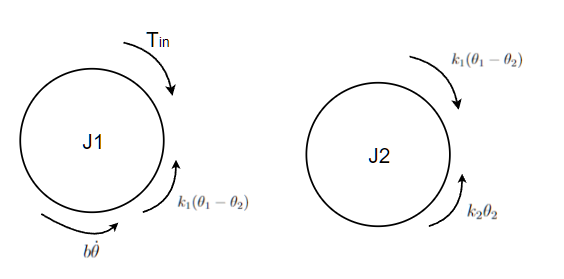
\includegraphics[scale = 0.9]{images/q1_DCL_J1-J2.png}
\label{filtro1}
\caption{Diagrama de Corpo Livre - J1 e J2}
\end{figure}\\

Portanto, teremos para J1:


\begin{equation}\label{eq_j1}
    J_1\ddot \theta_1 = T_{in} - b \dot \theta_1 - k_1(\theta_1 - \theta_2)
\end{equation}

Da mesma forma, para J2:

\begin{equation}\label{eq_j2}
    J_2\ddot \theta_2 = k_1(\theta_1 - \theta_2) - k_2 \theta_2
\end{equation}


Então, fazendo (\ref{eq_j1}) + (\ref{eq_j2}), teremos:

\begin{equation}
    \sum{T} = J_1 \ddot \theta_1 + J_2 \ddot \theta_2 = T_{in} - b \dot \theta_1 - k_1(\theta_1 - \theta_2) + k_1(\theta_1 - \theta_2) - k_2 \theta_2
\end{equation}\\

Por fim, podemos simplificar e obtemos nosso modelo matemático:

\begin{equation}
    T_{in} = J_1\ddot \theta_1 + J_2\ddot \theta_2 + b\dot \theta_1 + k_2 \theta_2 
\end{equation}

\newpage
\section{Questão 02}
A figura abaixo mostra um sistema pêndulo simples com duas molas de constante de rigidez $k$. A massa m do pêndulo está concentrada na sua extremidade. Assuma que a força da mola exercida no pêndulo é nula quando ele está na vertical. Assuma também que o atrito é desprezível e o ângulo de oscilação é pequeno. O pêndulo possui comprimento total $L$, e a distância do topo do pêndulo até a linha das molas é a. A velocidade inicial do pêndulo é nula.

\begin{figure}[H]
\centering

\includegraphics[scale = 0.7]{images/sistema2.png}
\label{filtro1}
\caption{Sistema pendulo simples - questão 02}
\end{figure}

\subsection{Modelo Matemático do Sistema}

Sabemos que há dois torques agindo neste sistema, sendo um deles devido à força da gravidade e o outro devido à força da mola. Então, a princípio, para a equação de movimento para este sistema, considerando a Segunda Lei de Newton, teremos:

\begin{equation}\label{eq1_q2-a}
    J \ddot \theta = -mgl\sin{\theta} - 2(ka\sin{\theta})(a\cos{\theta})
\end{equation}

Onde sabemos que

\begin{equation}
    J = ml^2
\end{equation}

Portanto, reescrevendo a eq. \ref{eq1_q2-a}, obtemos o nosso modelo matemático, ainda que não linearizado:

\begin{equation}\label{eq3_q2-a}
    ml^2 \ddot \theta + mgl \sin{\theta} + 2 ka^2 \sin{\theta}\cos{\theta} = 0
\end{equation}

\begin{equation}\label{eq3_q2-a}
     \ddot \theta  = \sin{\theta}(\frac{- g }{l} - \frac{2 ka^2\cos{\theta}}{ml^2})
\end{equation}



\subsection{Linearização}
Considerando a aproximação de ângulos pequenos, onde teríamos $\sin{\theta}=\theta$ e $\cos{\theta} = 1$, podemos simplificar nossa equação \ref{eq3_q2-a} e, assim, obtemos nosso modelo matemático do sistema \textbf{linearizado}:

\begin{equation}\label{eq3_q2-a}
     \ddot \theta  = - \theta(\frac{ g }{l} + \frac{2 ka^2}{ml^2})
\end{equation}


\subsection{Resposta Dinâmica do Sistema - Simulink}
Encontrar a resposta dinâmica do sistema (ângulo do pêndulo em função do tempo) usando o Simulink, a partir do modelo matemático linearizado.

\begin{figure}[H]
\centering
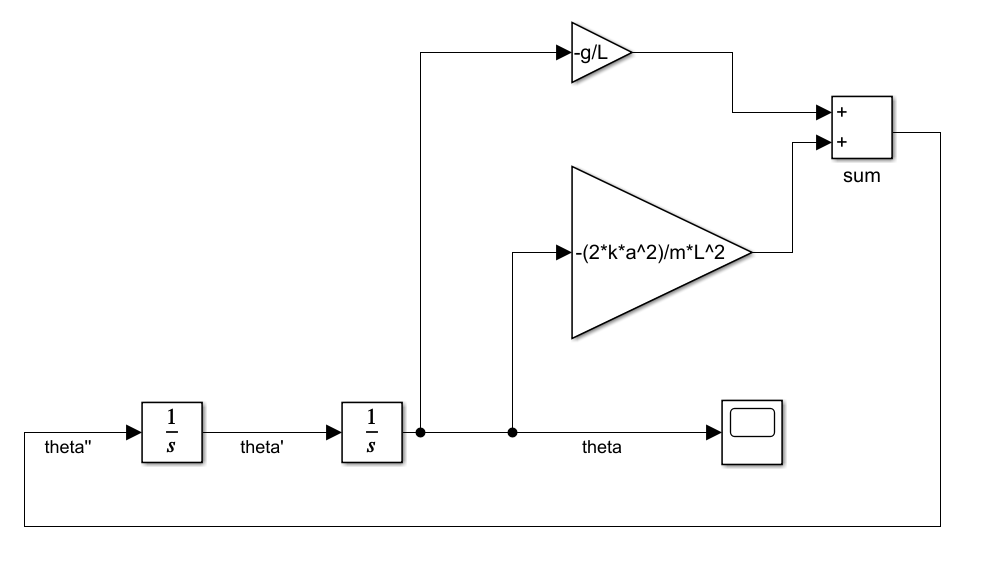
\includegraphics[scale = 0.6]{images/q2_sistema_simulink.png}
\label{filtro1}
\caption{Resposta Dinâmica com Simulink}
\end{figure}

\subsection{Definição dos parâmetros}
Devemos criar um script no MATLAB para definir os parâmetros do sistema e rodar o Simulink. Feito isso, segue abaixo a demonstração do código gerado:

\sloppy
\epstopdfsetup{outdir=./}
\graphicspath{ {./L01_Latex_images/} }


\begin{matlabcode}
%% Lista 4 - questão 2
close all
clear
clc

%definição dos parâmetros

% Sistema pendulo simples

theta_0 = 0.01;  %rad
k = 10;          %N/m
a = 0.6;         %m
L = 1;           %m
m = 1;           %kg
g = 9.8;         %m/s^2

\end{matlabcode}

\subsection{Resposta Gráfica}

No script criado, devemos gerar os gráficos de posição/velocidade do pêndulo em função do tempo, usando os parâmetros iniciais:\\

$theta0 = 0.01 rad$\\
$k = 10 N/m$\\
$a = 0.6 m$\\
$L = 1 m$\\
$m = 1 kg$\\

No tópico anterior, foi feita a demonstração de código com estes mesmos parâmetros.

\begin{figure}[H]
\centering
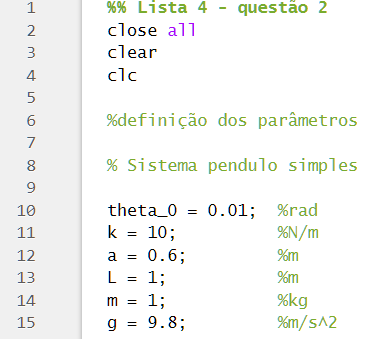
\includegraphics[scale = 0.7]{images/q2_matlab-code.png}
\label{filtro1}
\caption{Definição dos parâmetros no MATLAB}
\end{figure}

Portanto, podemos gerar o gráfico, ao fazermos o script compilar em paralelo com o sistema no Simulink:

\begin{figure}[H]
\centering
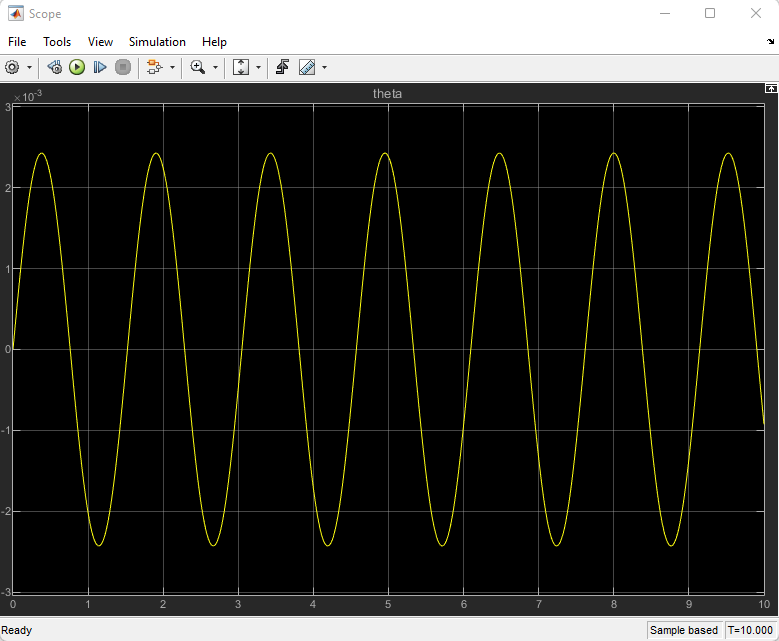
\includegraphics[scale = 0.65]{images/q2_graph.png}
\label{filtro1}
\caption{Gráfico da resposta dinâmica com o Simulink}
\end{figure}

\subsection{Aumento da constante das molas}
Neste tópico, aumentaremos a constante $k$ para 100 N/m e verificaremos o que acontece com o gráfico.

\begin{figure}[H]
\centering
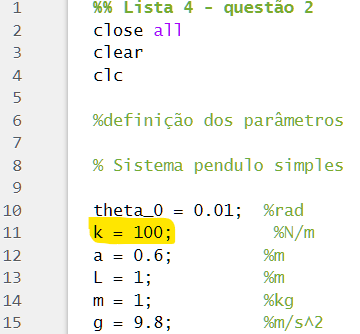
\includegraphics[scale = 0.65]{images/q2_k-redefinido-100.png}
\label{filtro1}
\caption{Script - Redefinição do parâmetro K para 100 N/m}
\end{figure}

\begin{figure}[H]
\centering
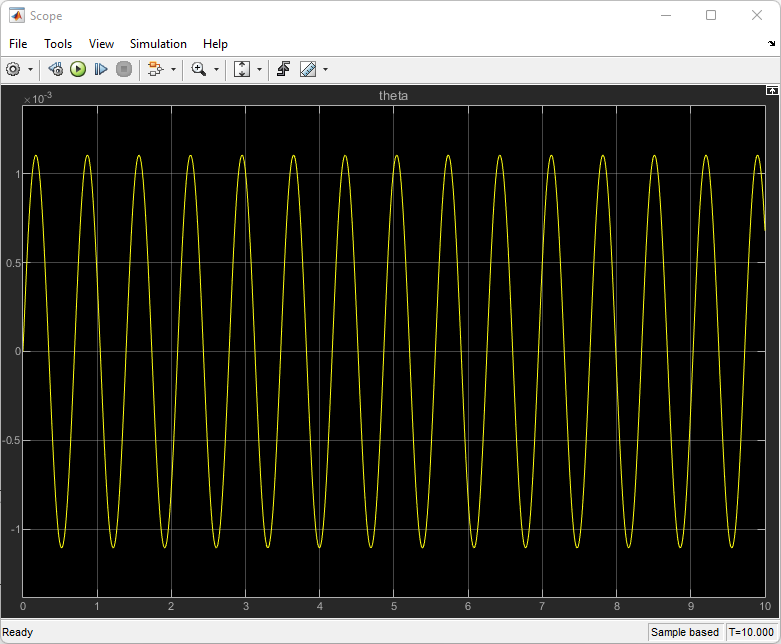
\includegraphics[scale = 0.65]{images/q2_graph2_k-100.png}
\label{filtro1}
\caption{Gráfico da resposta dinâmica com o Simulink com k=100N/m}
\end{figure}

Percebemos um aumento periódico no gráfico, isto é, nas oscilações. Portanto, podemos dizer que o comportamento está coerente, já que, de acordo com as leis do Movimento Harmônico Simples, a frequência é diretamente proporcional à constante elástica da mola, ou seja, quanto mais rígida for esta mola, mais rápido será o movimento oscilatório do sistema.

\newpage
% REFERENCIAS %%%%%%%%%%%%%%%%%%%%%%%%%%%%%%%%%%%%%%%%%%%%%%%%%%%%%%%%%%%%%%
    \nocite{*}
    \bibliography{src/bibliography}
    
\end{document}
\section{Referências Bibliográficas}



\end{document}